\section{Applying Gaussian Processes to Astrostatistics}
% Possible domains:
% 
% 
% Materials science \cite{materials}
% 
% 
% Cosmography \cite{cosmography}
% 
% 
% Statistical emulators \cite{emulators}
% 
% 
% Signals processing \cite{signals-processing}


\subsection{Introduction}

\subsubsection{SED modelling background}
The optical light from a distant galaxy, integrated over its entire size in the sky, comes from stars and gas in the galaxy that shine. We can find the spectral energy distribution (SED) of the galaxy by measuring the brightness at different wavelength bands. Brightness at specific wavelenghts can be used to infer the existence of certain behaviours in the galaxy's gases and stars. 

\begin{figure}[H]
	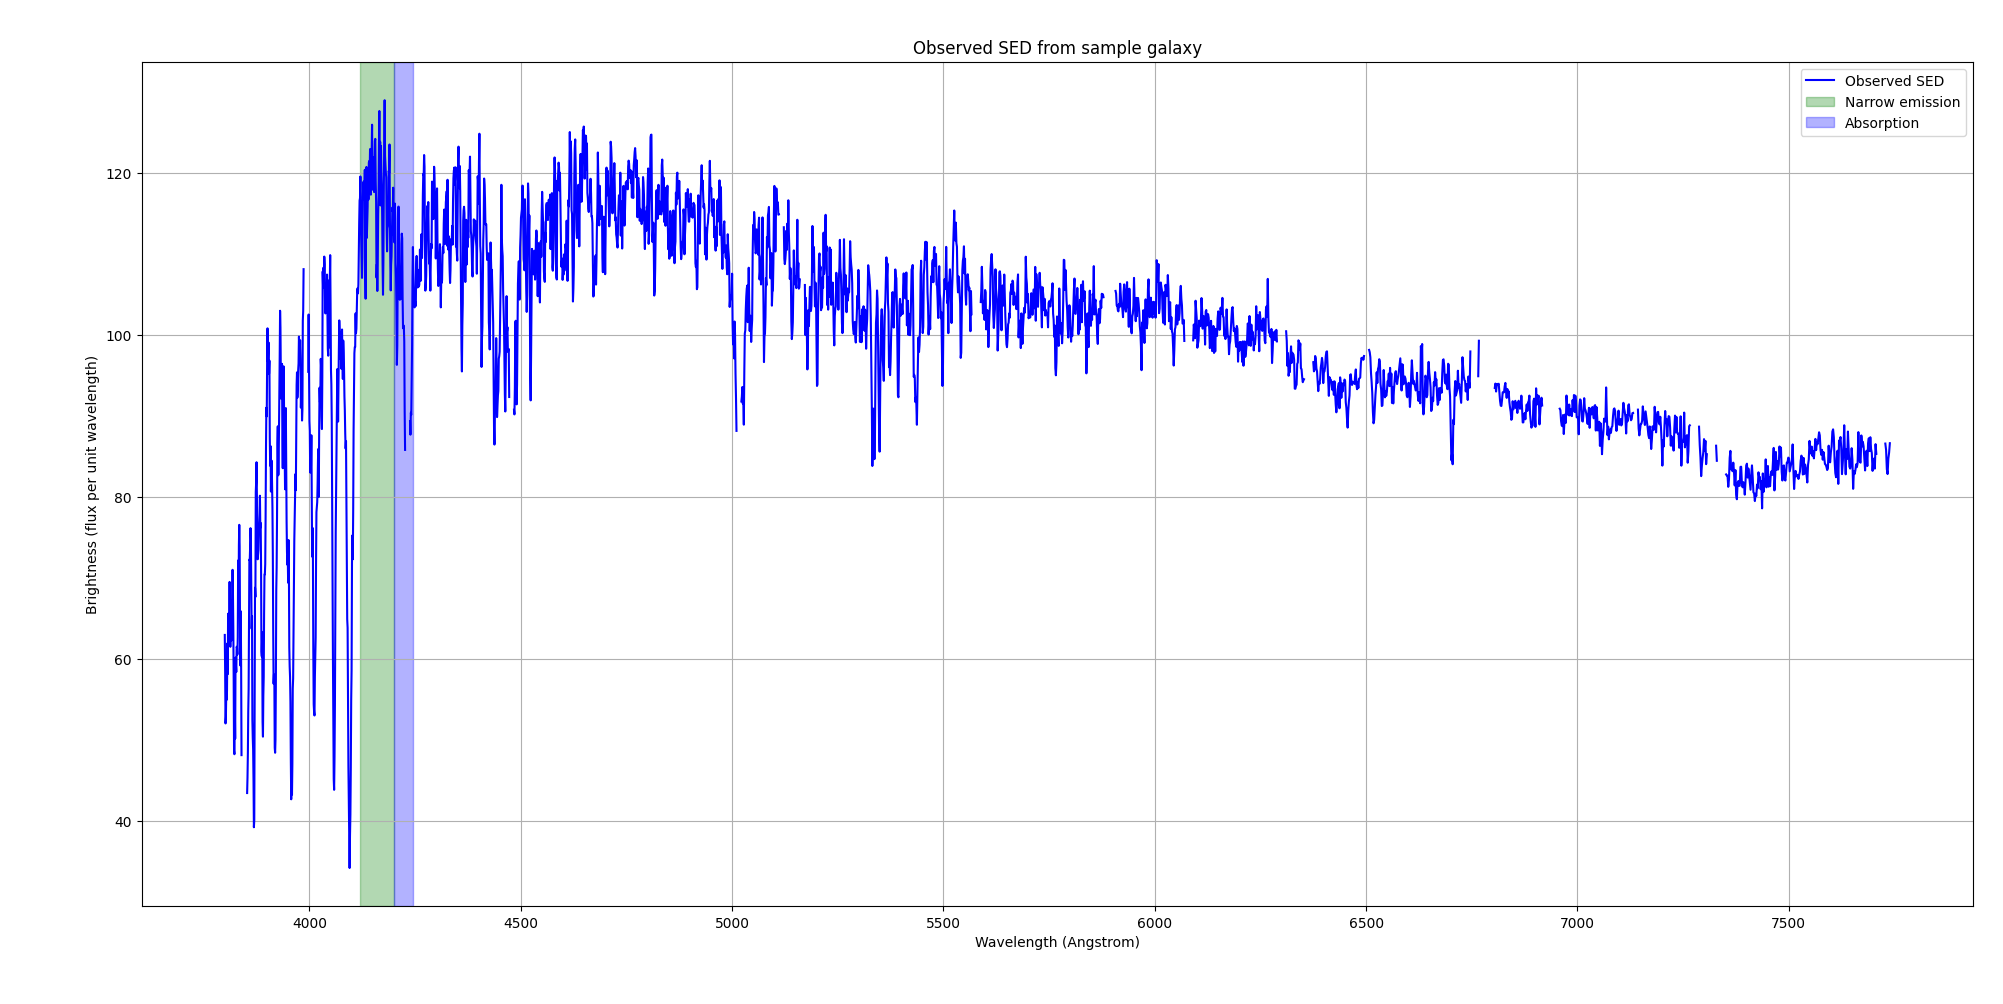
\includegraphics[height=0.5\textwidth]{application/observed-spectrum.png}
    \caption{SED of a sample galaxy (id 51613-0305-552) \cite{galaxy-gp-noise}.}
\end{figure}
The 4000-4500 wavelength region of this SED contains two examples of how a galaxy's age can be inferred after observing their SED. The upward narrow emission band highlighted in green is from ionised gas, mostly Hydrogen and Oxygen in this wavelength range, produced by younger stars. The downward dipping absorption band in red is from electronic transitions in the stars atmospheres, such as Hydrogen and Calcium, that occurs in older stars \cite{galaxy-spectra-101}. Astronomers use very complex models with many free parameters and hidden variables to understand the effect of characteristics of the stars and gases of the galaxy on the SED \cite{galaxy-spectra-101}.

\begin{figure}[H]
    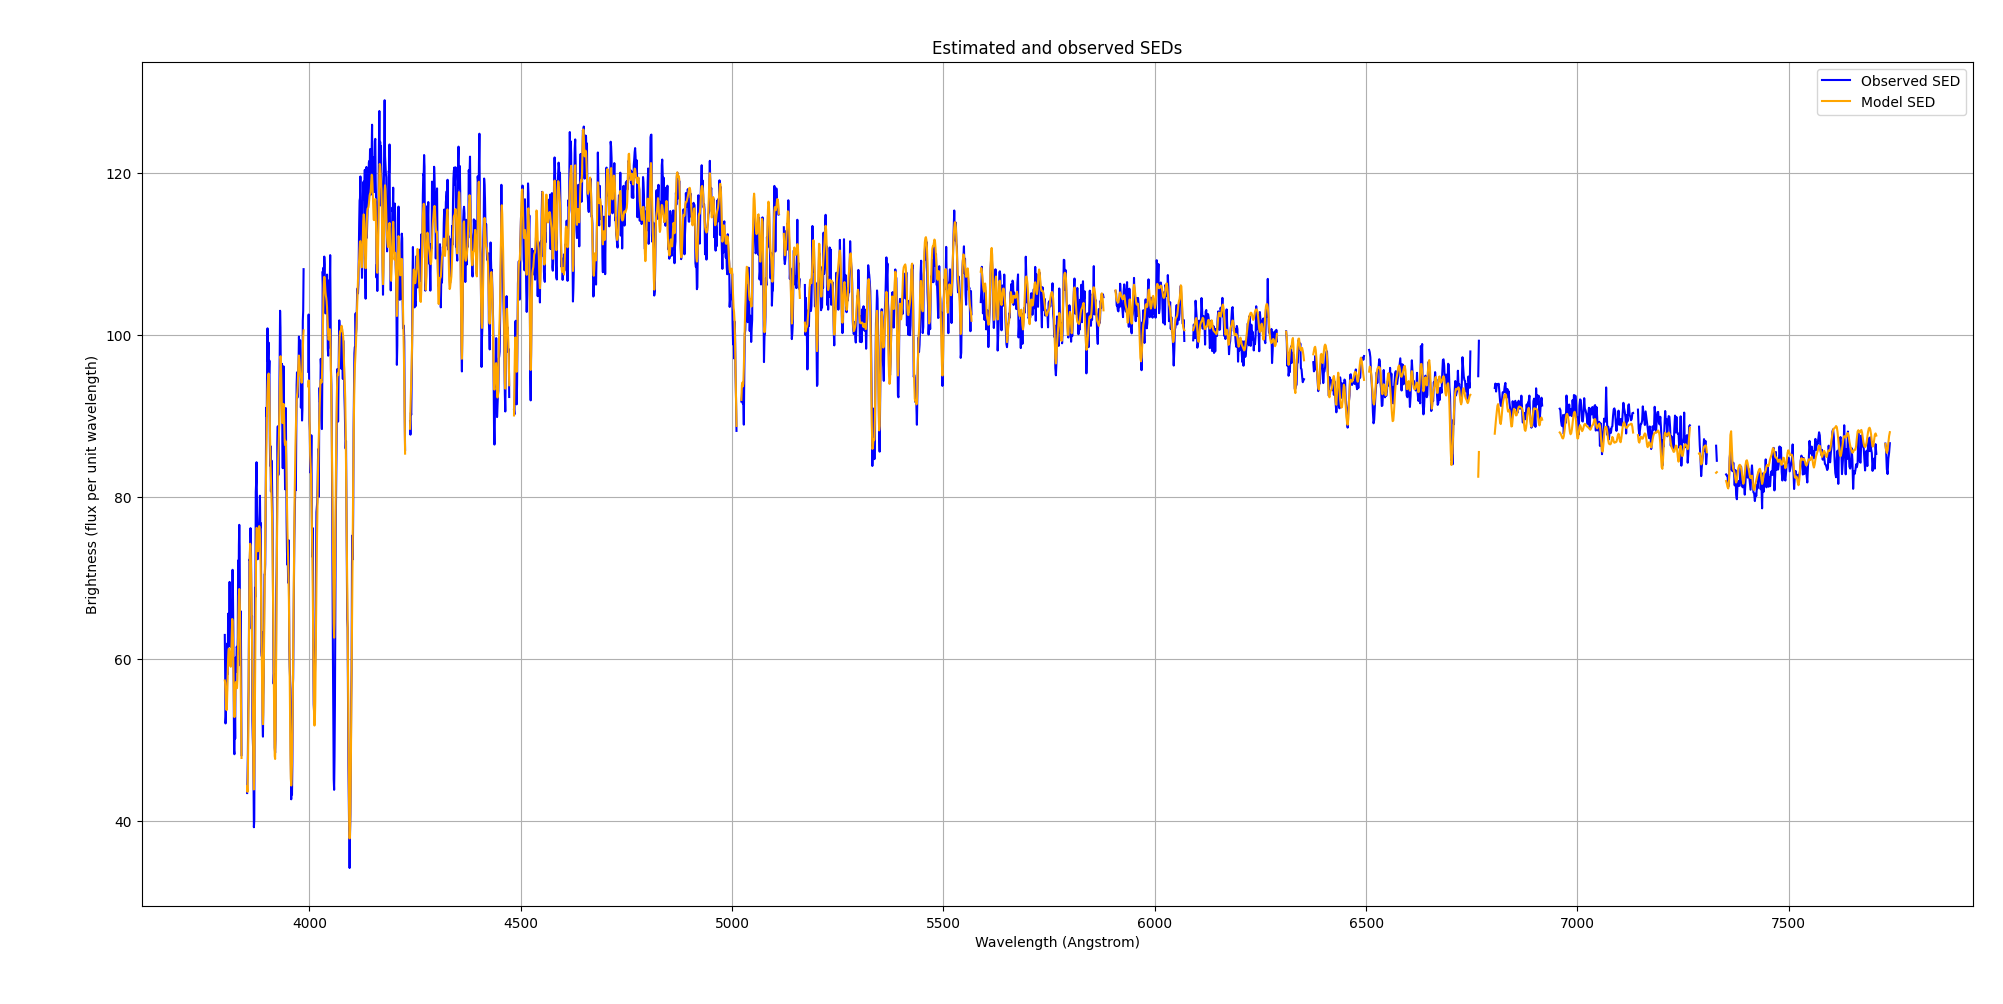
\includegraphics[height=0.5\textwidth]{application/model.png}
    \caption{SED estimated using Leung's model of the the sample galaxy alongside its observed SED \cite{galaxy-gp-noise}.}
\end{figure}
Leung's model \cite{galaxy-gp-noise} agreed with the observed SED in that the regions we identified as emissions and absorption bands but failed to predict brightness in other regions of the SED. In particular, large amounts of true emmissions were missed in a low wavelength region (<4500 Angstroms) and a high wavelength region (6500-7500 Angstroms), while the model predicted a large absorption band in the 4100 Angstrom region that did not exist.

\subsubsection{Low-frequency wobbles}
\begin{figure}[H]
    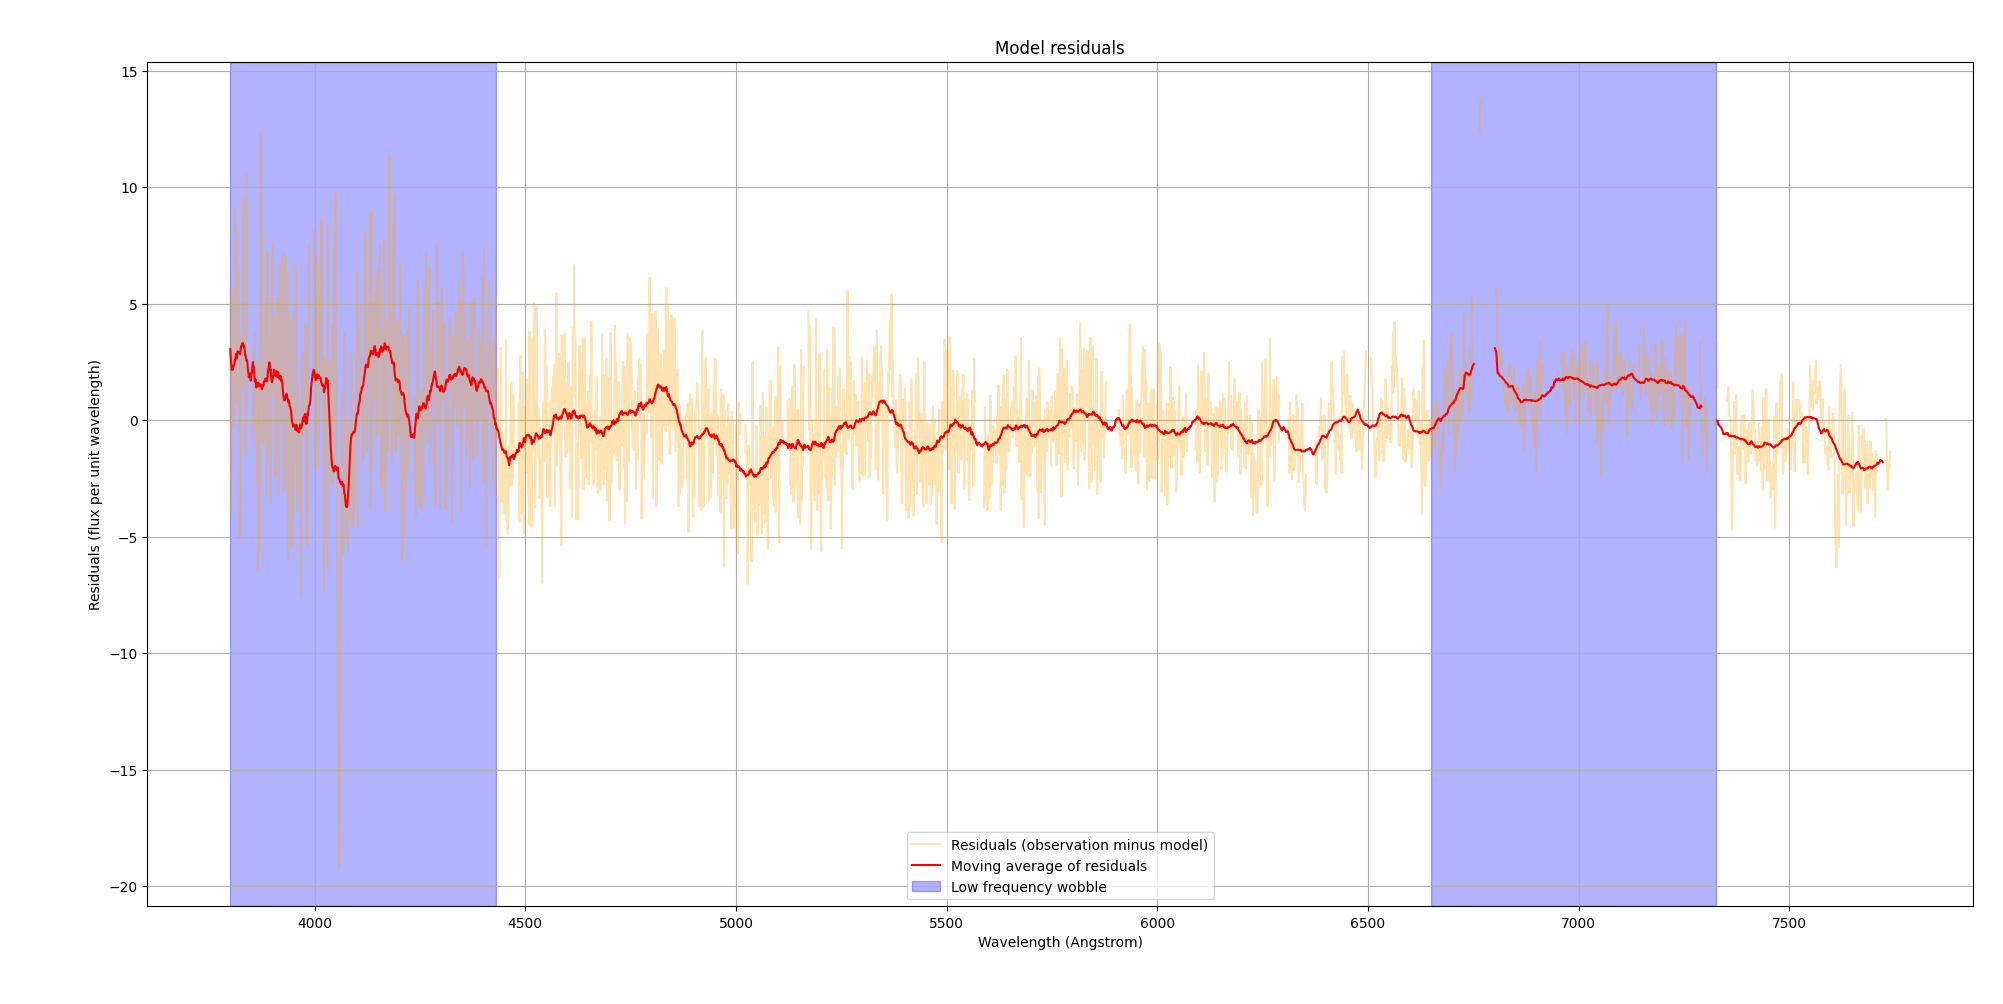
\includegraphics[height=0.5\textwidth]{application/raw_residuals.png}
    \caption{Residuals of the model fit to the SED of the same galaxy \cite{galaxy-gp-noise}.}
\end{figure}
Residuals that behave as zero-mean noise are dependent on how long we observe the galaxy for and are not of interest \cite{galaxy-spectra-101}. However, the two regions identified previously are reflected in the model's residuals - the residuals oscillate above zero in the low and high wavelength regions, with the exception of the 4100 Angstrom negative residual spike. We refer to these regions as low frequency wobbles because these oscillations occur at a lower frequency than the oscillations around zero in the remaining SED.SED models exhibiting low-frequency wobbles are problematic to use for inference as they violate the zero-mean noise assumption \ref{eq:model_error_assumption}, leading to biased estimates of the model parameters and their uncertainties.

% A low frequency wobble has two sources: problems with the data reduction process, and problems with the model. We can seperate these sources by modelling large numbers of galaxies that differ greatly in their distance to Earth. Light from farther galaxies that takes longer to reach us exhibits is shifted to longer wavelengths - aphenomenon called "redshift",  due to the expansion of the universe. Low frequency wobbles caused by data reduction problems will occur in the same observed wavelength region for all galaxies, while low frequency wobbles caused by the model will occur in different observed wavelength regions \cite{galaxy-spectra-101}.

As the source of low-frequency wobbles is not well understood and cannot be incorporated into an SED model \cite{galaxy-spectra-101}, we need a method to remove these low-frequency wobbles without altering or biasing the high-frequency noise that is required for inference (e.g. standard errors in frequentist regression). Signals processing methods would require a fixed frequency cutoff, which does not exist as the amplitude and scale of the low-frequency wobbles vary between galaxies and needs to be learned from the data. Although large non-parametric models (e.g. neural networks) could learn from data, both methods produce point estimates of residuals, the uncertainty of which cannot be propagated through to the SED model parameters and used for inference.

\subsection{Methodology}
\subsubsection{Using GPs for SED residual modelling}
\begin{figure}[H]
    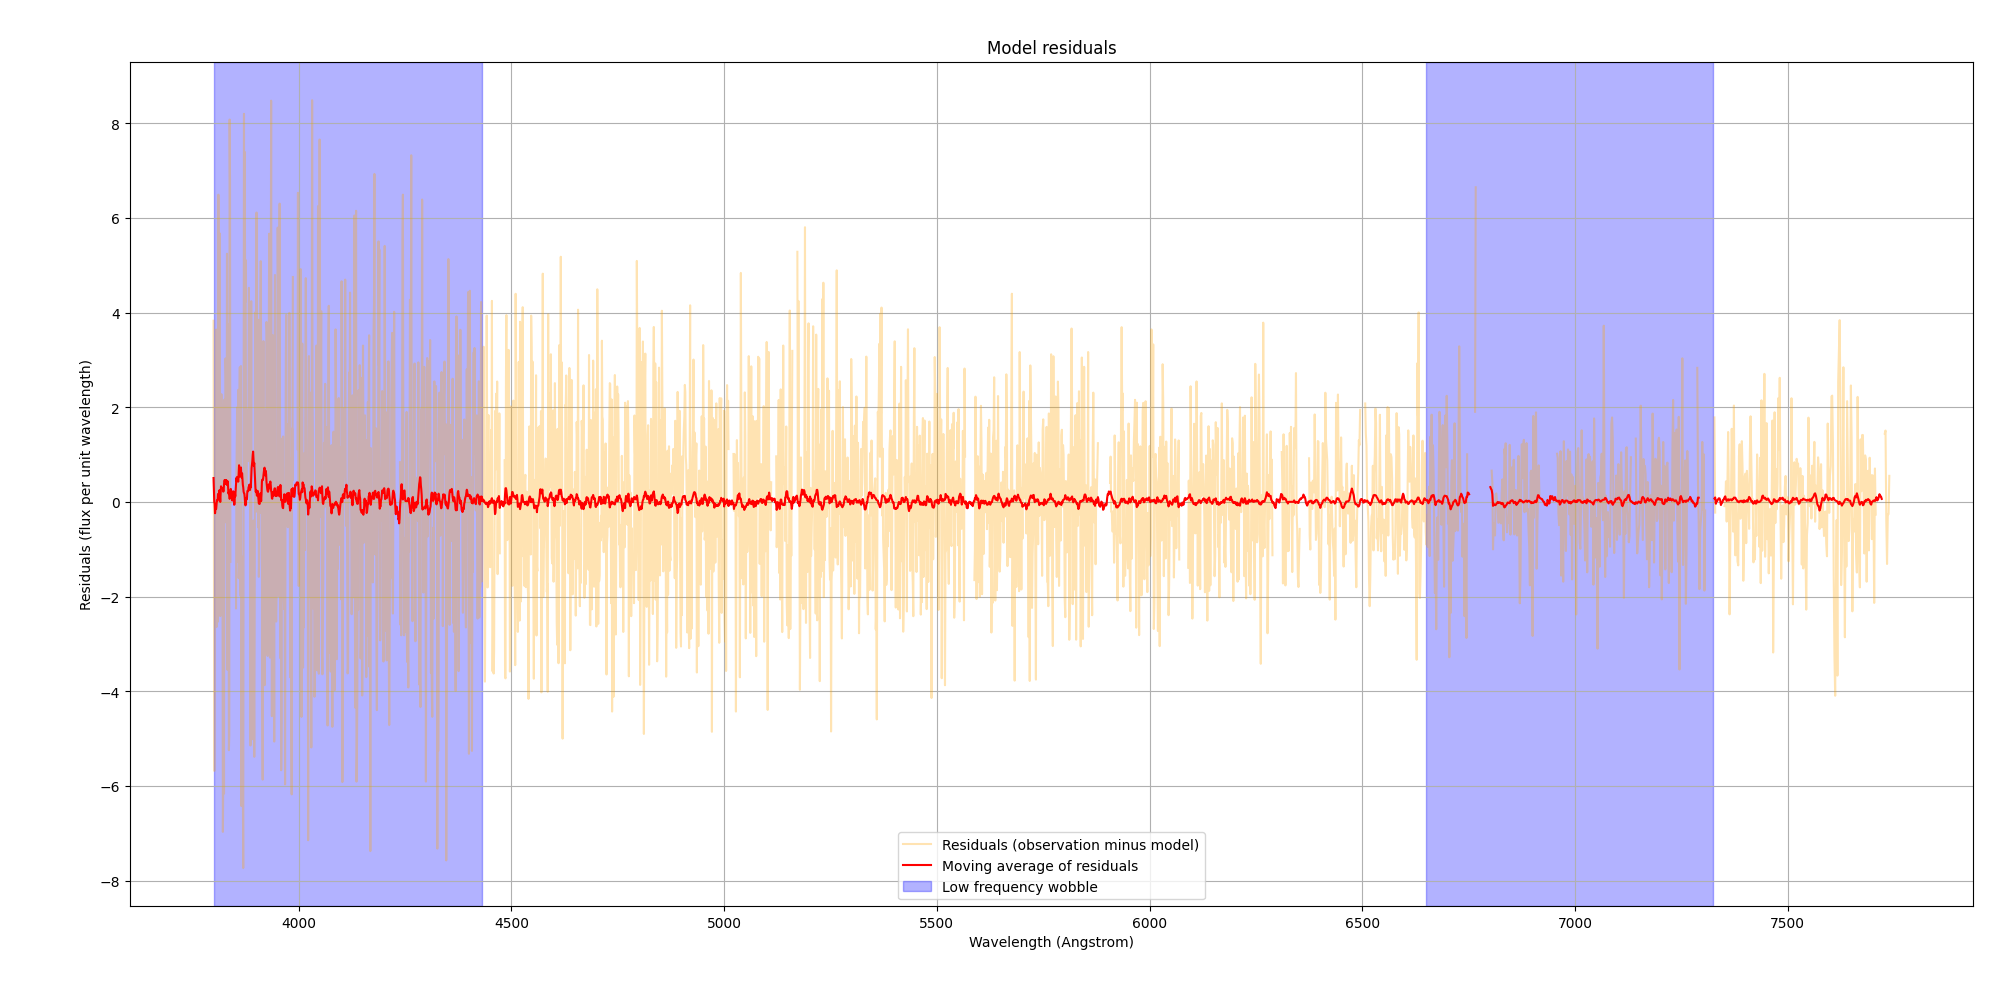
\includegraphics[height=0.5\textwidth]{application/gp_residuals.png}
    \caption{Remaining residuals after fitting a full GP using SE \cite{galaxy-gp-noise} to the raw residuals of the previous SED model.}
\end{figure}
GPs are a natural choice for this problem as they can identify the low-frequency wobbles on a per-galaxy basis, whilst doing so in a probabilistic framework that allows the uncertainty in this estimation to be propagated. SE \ref{eq:se} is likely the best kernel for SED modelling because its spectral density converges to zero faster than any other kernel, meaning it ignores high-frequency noise more than other kernels. 

Unfortunately, GPs have a naive training and inference cost of $O(n^3)$ and each SED data contains thousands of data points (e.g. the example galaxy has 3000 data points), which makes training and inference on a single galaxy infeasible. 

\subsubsection{Approximations and kernels considered}
We compare two methods of addressing this cubic complexity to enable the use of GPs for SED residual modelling on large numbers of galaxies. SVGP is an approximation-based method that sacrifices accuracy, computational complexity and wall-clock speed in exchange for generality. SVGPs can be used with any kernel and can be applied to any dataset \cite{svgp}. Conversly, a celerite speedup achieves near-perfect accuracy and significant improvements in computational complexity and wall-clock speed, but can only be used with Matern 3/2 kernels and on particular datasets \cite{foreman-mackay}. Although this dataset meets all the conditions for celerite models (one dimensional and data is sorted by wavelength), using a rougher kernel like Matern 3/2 will capture too much noise compared to SE. We determine if the overfitting from using Matern 3/2 outweighs the computational gains from using celerite.

% https://gpy.readthedocs.io/en/deploy/ \cite{gpy}

% https://celerite2.readthedocs.io/en/latest/ \cite{foreman-mackay}

\subsection{Results}

\begin{figure}[H]
    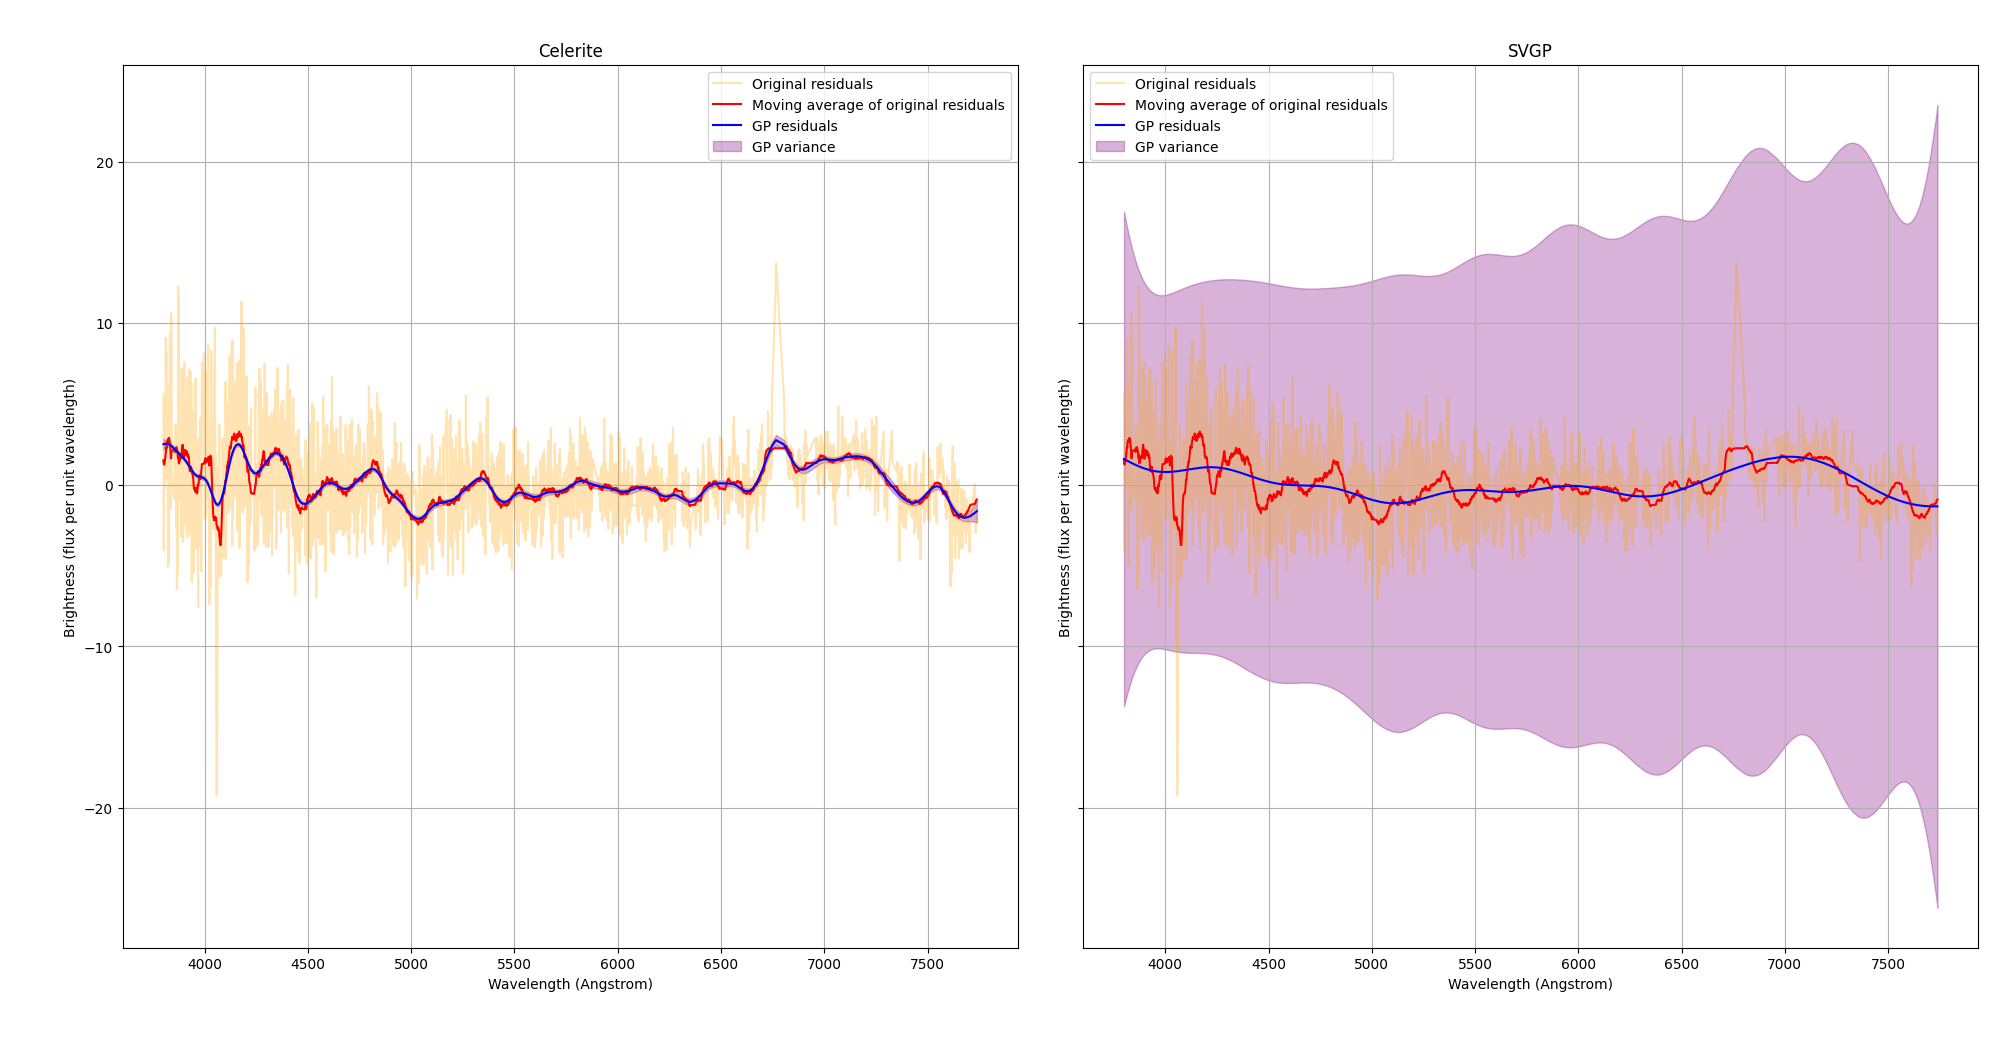
\includegraphics[height=0.5\textwidth]{application/celerite_svgp.png}
    \caption{Comparison of the residuals produced by GPs using different kernels and approximation methods to Leung's SED model \cite{galaxy-gp-noise}. SVGP was trained using the SE kernel, while celerite was trained using the Matern 3/2 kernel.}
\end{figure}
Matern 3/2 ultimately performed worse on this task because it produced a GP whose expected function draw oscillated too much around zero in high frequency regions, unlike SE which remained at zero in high frequency regions but rose in the low frequency regions. Thus, Matern 3/2 overfitted to the data while SE captured the low frequency wobbles without overfitting. 

% The variance in SE is much larger than the variance in Matern 3/2 and rise with wavelength. This reflects the tendancy for high-frequency noise to increase with wavelength \cite{galaxy-spectra-101}.

% SVGP SE: Training: 2262.48 seconds, Inference: 0.02 seconds
% Celerite Matern 3/2: Training: 0.01 seconds, Inference: 0.84 seconds

\begin{table}[H]
    \centering
    \begin{tabular}{|c|c|c|c|c|c|}
        \hline
        Kernel & Approximation & Theoretical complexity & Training time (s) & Inference time (s) & Epochs \\
        \hline
        SE & SVGP & $O(bm^2 + m^3)$ & 2262.48 & 0.02 & 2500 \\
        \hline
        Matern 3/2 & Celerite & $O(n)$ & 0.01 & 0.84 & 10 \\
        \hline
    \end{tabular}
    \caption{Comparison of the training and inference times of SVGP and celerite approximations to Leung's SED model \cite{galaxy-gp-noise}. Theoretical complexities are given in terms of dataset size $n$, batch size $b$ and number of inducing points $m$.}
\end{table}
SVGP took 65,000 times longer and 250 times more epochs to converge than celerite.

\subsection{Discussion}
\subsubsection{Computational cost}
In total, SVGP required 15 billion operations to complete its training cycle. This incredible cost was largely caused by SVGP's sensitivity to the noise in the dataset, which in turn raised the per-epoch cost and number of epochs required to converge.

% massive number of inducing points and batch size
SVGP's $O(bm^2 + m^3)$ training complexity appears theoretically attractive due to its lack of dependence on dataset size $n$. However, the noise of this dataset raised the number of inducing points (min. 256) and batch sizes (1024) required to produce a subset of the data that was representative enough for the model to learn from. This directly raised the number of operations required per epoch to a minimum of 80 million operations, in contrast to celerite's $O(n)$ training complexity only necessitatating 3000 operations per epoch.

% more parameters to optimise
Furthermore, the raised $m$ and batch size meant the optimiser required far more epochs to converge on the optimal parameters compared to celerite. Celerite is only optimising two kernel parameters, signal noise $\sigma_s^2$ and length scale $l$, while SVGP has to additionally optimise a full set of variational parameters for the SVGP posterior \label{eq:svgp_posterior} for each inducing point. Thus, the increase in $m$ necessitated by noise also increased the difficulty of the optimisation problem, which meant that SVGP took 2500 epochs to converge compared to celerite's ten epochs.

\subsubsection{Overfitting}
Similar to its behaviour on the toy datasets, Matern 3/2 is a rough process and its expected function draw passes through all the datapoints. This is an undesireable property for SED residual modelling, as it means that the GP will capture both high and low frequency noise. In contrast, SE's highly limited flexibility disincentivises it from modelling the noise in favour of approaching the large number of points in the low-frequency wobble regions. This is similar to its behaviour on the smooth toy dataset, where SE avoided one stray point so its expected function draw could get closer to two other points.

\subsection{Conclusion}
% computational
% svgp is unusably slow
% test svgp on gpu
SVGP is not a suitable method for SED residual modelling because of its extreme computational cost. However, SVGP's batching and use of an iterative optimiser means it lends itself well to GPU processing are supported by more recent SVGP implementations such as GPyTorch \cite{gpytorch} and GPFlow \cite{gpflow}. Training SVGP on a GPU using these frameworks could significantly reduce its training time. 

% numerical accuracy issues
% fit both with Matern 3/2 to compare SVGP accuracy degredation
Another issue with SVGPs that was not explored in this work is their inherent inaccuracy compared to celerite or more analytical ELBO methods such as VFE. If GPUs make SVGP computationally feasible, we would need to determine if the accuracy degradation is acceptable for SED residual modelling since a high accuracy degredation could introduce additional errors into the high frequency noise, which would bias the SED model parameters and their uncertainties.

% overfitting
% matern 3/2 overfits
Although celerite was highly computationally performant on this dataset, its inability to use SE means it is not suitable for SED residual modelling. It can only use Matern 3/2's kernel, and this kernel's roughness means it overfits to the data and removes both high and low frequency noise. A naive approach would be to artificially increase the length scale of Matern 3/2 to increase its rate of spectral decay \ref{eq:matern_spectral} and mimic SE's behaviour. While this would achieve the desired behaviour of removing low frequency wobbles without removing high frequency noise, this would likely produce worse estimates of SED residuals than SE.

% blast matern's length scale \ref{eq:matern_spectral} in exchange for worse GP
% other structured approximations with linear cost that can produce 1D SE
% create SE from celerite
